% For LaTeX-Box: root = stat305-pexam1.Rnw
\documentclass[addpoints]{examsetup}

\usepackage{etoolbox}
\usepackage{tikz,pgfplots}

%% For LaTeX-Box: root = stat105_exam1_info.tex 
%%%%%%%%%%%%%%%%%%%%%%%%%%%%%%%%%%%%%%%%%%%%%%%%%%%%%%%%%%%%%%%%%%%%%%%%%%%%%%%%
%  File Name: stat105_exam1_info.tex
%  Purpose:
%
%  Creation Date: 24-09-2015
%  Last Modified: Thu Sep 24 13:51:36 2015
%  Created By:
%%%%%%%%%%%%%%%%%%%%%%%%%%%%%%%%%%%%%%%%%%%%%%%%%%%%%%%%%%%%%%%%%%%%%%%%%%%%%%%%
\newcommand{\course}[1]{\ifstrempty{#1}{STAT 105}{STAT 105, Section #1}}
\newcommand{\sectionNumber}{B}
\newcommand{\examDate}{October 1, 2015}
\newcommand{\semester}{FALL 2015}
\newcommand{\examNumber}{II}

\newcommand{\examTitle}{Exam \examNumber}

\runningheader{\course{\sectionNumber}}{Exam \examNumber}{\examDate}
\runningfooter{}{}{Page \thepage of \numpages}

\newcommand{\examCoverPage}{
   \begin{coverpages}
   \centering
   {\bfseries\scshape\Huge Exam I \par}
   \vspace{1cm}
   {\bfseries\scshape\LARGE \course{\sectionNumber} \par}
   {\bfseries\scshape\LARGE \semester \par}

   \vspace{2cm}

   \fbox{\fbox{\parbox{5.5in}{\centering 

      \vspace{.25cm} 
      
      {\bfseries\Large Instructions} \\

      \vspace{.5cm} 

      \begin{itemize}
         \item  The exam is scheduled for 80 minutes, from 8:00 to 9:20 AM. At 9:20 AM the exam will end.\\
         \item  A forumula sheet is attached to the end of the exam. Feel free to tear it off.\\
         \item  You may use a calculator during this exam.\\
         \item  Answer the questions in the space provided. If you run out of room, continue on the back of the page. \\
         \item  If you have any questions about, or need clarification on the meaning of an item on this exam, please ask your instructor. No other form of external help is permitted attempting to receive help or provide help to others will be considered cheating.\\
         \item  {\bfseries Do not cheat on this exam.} Academic integrity demands an honest and fair testing environment. Cheating will not be tolerated and will result in an immediate score of 0 on the exam and an incident report will be submitted to the dean's office.\\
      \end{itemize}

   }}}

   \vspace{2cm}

   \makebox[0.6\textwidth]{Name:\enspace\hrulefill}

   \vspace{1cm}

   \makebox[0.6\textwidth]{Student ID:\enspace\hrulefill}
   \end{coverpages}

}


\newcommand{\course}[1]{\ifstrempty{#1}{STAT 305}{STAT 305, Section #7}}
\newcommand{\sectionNumber}{3}
\newcommand{\examDate}{February 6, 2020}
\newcommand{\semester}{Spring 2020}
\newcommand{\examNumber}{I}

\usepackage{Sweave}
\begin{document}
\Sconcordance{concordance:stat305-exam1.tex:stat305-exam1.Rnw:%
1 13 1 1 0 3 1 1 9 36 1 1 4 52 1 2 2 68 1 6 3 4 1 1 32 4 1 1 3 11 0 1 3 %
30 1 2 2 9 1 1 7 17 1 2 2 9 1}


%-- : R code (Code in Document)


\examCoverPage

\begin{questions}

\question[2] 
Circle the \textbf{bold face} term that makes the following statement true: \\

A measurement device that reports the measurements which are close to each other when repeatedly measuring the same thing is (\textbf{precise} or \textbf{accurate}).
\vspace{1cm}

\question[2] 
A number of issues concerning measurement must be addressed in the following order:\vspace{0.2cm}\\

(1) precision, validity, accuracy \hspace{1cm} (2) accuracy, precision, validity\\
(3) validity, accuracy, precision \hspace{1cm} (4) validity, precision, accuracy

\vspace{1cm}

\question[2]
For a complete(full) factorial study with three factors, each with 4 levels, the number of all possible combinations (i.e the least number of observation) is:\vspace{0.2cm}\\

(1) 12\hspace{0.5cm} (2) 64\hspace{0.5cm} (3) 81\hspace{0.5cm} (4) none of these

\vspace{3cm}

\question[2]
In a series of experiments to study the priority of a chemical product, the reactor temperature is set fixed at $550$\textdegree C. The variable "reactor temperature" is a \vspace{0.2cm}\\

(1) response variable\hspace{1cm} (2) controlled variable\\
(3) blocking variable\hspace{1cm} (4) experimental variable
\vspace{1cm}
\pagebreak

\question
%-- : R code (Code in Document)

A sample of size 6 was drawn from a population and the resulting observations are reported below. 
\begin{center}
110, 100, 105, 103, 105, 115
\end{center}
Using these observed values, report the following:
\vspace{1cm}

\begin{parts}

   \part[2] the mean  
   \hfill \fbox{ \textcolor[rgb]{1.00,1.00,1.00}{$\bigcap$} \hskip-0.4cm $\bar{x}=$ \hspace{2cm}}
   \vspace{3cm}



   \part[3] the median 
      \hfill \fbox{ \textcolor[rgb]{1.00,1.00,1.00}{$\bigcap$} \hskip-0.4cm $Med.=$ \hspace{2cm}}

   \vspace{3cm}

   \part[5] the variance 
      \hfill \fbox{ \textcolor[rgb]{1.00,1.00,1.00}{$\bigcap$} \hskip-0.4cm $s^2=$ \hspace{2cm}}

   \vspace{4cm}

   \part[2] the standard deviation 
      \hfill \fbox{ \textcolor[rgb]{1.00,1.00,1.00}{$\bigcap$} \hskip-0.4cm $s=$ \hspace{2cm}}

   \vspace{2cm}
   
   \part[3] the value of $Q(.75)$
         \hfill \fbox{ \textcolor[rgb]{1.00,1.00,1.00}{$\bigcap$} \hskip-0.4cm $Q(.75)=$ \hspace{2cm}}

   \vspace{4cm}

   \part[4] the interquartile range
            \hfill \fbox{ \textcolor[rgb]{1.00,1.00,1.00}{$\bigcap$} \hskip-0.4cm $IQR=$ \hspace{2cm}}

   \vspace{4cm}
   
   \part[5] give the coordinates (on a regular graph paper) of the upper right and lower left point that would appear on a normal plot of the data.

\hfill \fbox{upper right point = $( \;\;  \;\;  \;\; , \;\;  \;\;
\;\; )$ }

\hfill \fbox{lower left point = $( \;\;  \;\;  \;\; , \;\;  \;\;
\;\;  )$}

   \vspace{6cm}      
   \part[5] Using the axes below, create a box plot to summarize the data. Carefully label the axes
\centering   
%-- : R plot (results in document)
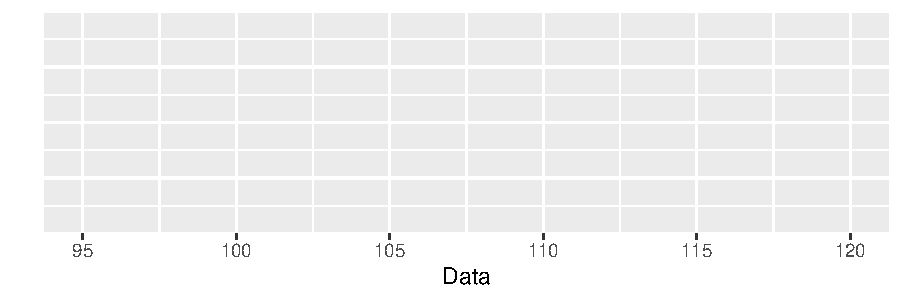
\includegraphics{stat305-exam1-003}
   \vspace{6cm}

\end{parts}

\pagebreak

\question

An environmental engineer is testing four methods for reducing the concentration of a certain lake pollutant found in Iowa lakes.
To do this he first randomly selected 20 Iowa lakes from which he took water samples,
then split each of the 20 samples into 4 portions, 
and randomly labeled the four portions 1, 2, 3, and 4. 
Finally, he attempted to reduce the concentration of each 
of the portions labeled 1 using the the first method, 
of each of the portions labeled 2 using the second method, 
of each of the portions labeled 3 using the third method, 
and of each of the portions labeled portion 4 using the fourth method. 
After the methods had been applied, he measured the change in concentration. \\

\begin{parts}
   \part[3] Is this an experiment or an observational study? Explain.

  \vspace{3cm}
  
    \part[2] What is the population under study?

  \vspace{3cm}

    \part[2] What is the sample under study?

  \vspace{3cm}

   \part Identify the following (if there was not one, simply put "not used").

  \vspace{1cm}

   \begin{subparts}
      \subpart[2] Response variable(s):

      \vspace{2cm}

      \subpart[2] Experimental variable(s):

      \vspace{2cm}
      
      \subpart[2] What type of variable was (were) the experimental variable(s) in previous question (circle one):\\
      
      \textbf{Quantitative}\hspace{2cm} \textbf{Qualitative}

      \vspace{2cm}

      \subpart[2] Blocking variable(s):

      \vspace{2cm}

   \end{subparts}

   \part[4] Was replication used in this experiment? If so, where was it applied? If not, how could we have applied it?

  \vspace{2cm}

\end{parts}

\pagebreak













\question
%-- : R code (Code in Document)

A certain make of load bearing beam used in construction of large buildings is certified to withstand pressures of 2.5 tonnes per square inch.
30 beams were tested and the pressures at which they failed are collected in the table below.

%-- : R code (Code in Document)
\begin{Schunk}
\begin{Soutput}
  The decimal point is at the |

  1 | 4
  2 | 8
  3 | 
  4 | 2555778899999
  5 | 01122222234559
  6 | 5
\end{Soutput}
\end{Schunk}

Note that \verb!0 | 9! represents 0.9. In this case, the first quartile is $Q(.25) = 4.7$, 
the median is 4.95, and the third quartile is $Q(.75) = 5.2$.

\begin{parts}
  \part[10] Complete the following frequency table: \\

  \begin{table}[h!]
     \centering
     \begin{tabular}{|l|p{3cm}|p{3cm}|p{4cm}|}
        \hline
                             & \textbf{Frequency} & \textbf{Relative} & \textbf{Cumulative}  \\
        \textbf{Value Range} &                    & \textbf{Frequency} & \textbf{Relative Frequency} \\\hline \hline
                    &  &  &  \\
      0.00 - 2.00   &  &  &  \\
                    &  &  &  \\ \hline
                    &  &  &  \\
      2.01 - 4.00   &  &  &  \\
                    &  &  &  \\ \hline
                    &  &  &  \\
      4.01 - 6.00   &  &  &  \\
                    &  &  &  \\ \hline
                    &  &  &  \\
      6.01 - 8.00   &  &  &  \\
                    &  &  &  \\ \hline
     \end{tabular}
  \end{table}

  \part[10] Using the axes below, create a box plot to summarize the data. Carefully label the axes.

%-- : R plot (results in document)
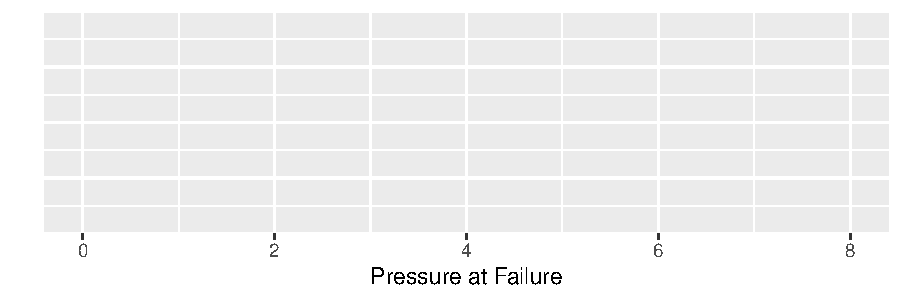
\includegraphics{stat305-exam1-012}

\newpage 

  \part[4] Are there any unusually low or high observations? If so, what pressures caused those beams to fail?

  \vspace{3cm}

  \part[10] The company also measured the heat at which the beams begin to deform (in 10,000 degrees Celsius). The values are collected below:

%-- : R code (Code in Document)

\begin{center}
   31.3, 41.8, 25.3, 35.3, 45.3, 37.3
\end{center}

Create a theoretical Q-Q plot using the following quantiles from the normal distribution as the theoretical quantiles. 
What does this graph tell us about the temperature at which the beams deform?

\begin{table}[h!]
   \centering
   \begin{tabular}{ccccccc}
             & 1 & 2 & 3 & 4 & 5 & 6  \\ \hline
      $p$    & 0.08 & 0.25 & 0.42 & 0.58 & 0.75 & 0.92 \\
      $Q_{N}(p)$ & -1.41 & -0.67 & -0.2 & 0.2 & 0.67 & 1.41 \\
   \end{tabular}
\end{table}

%-- : R plot (results in document)
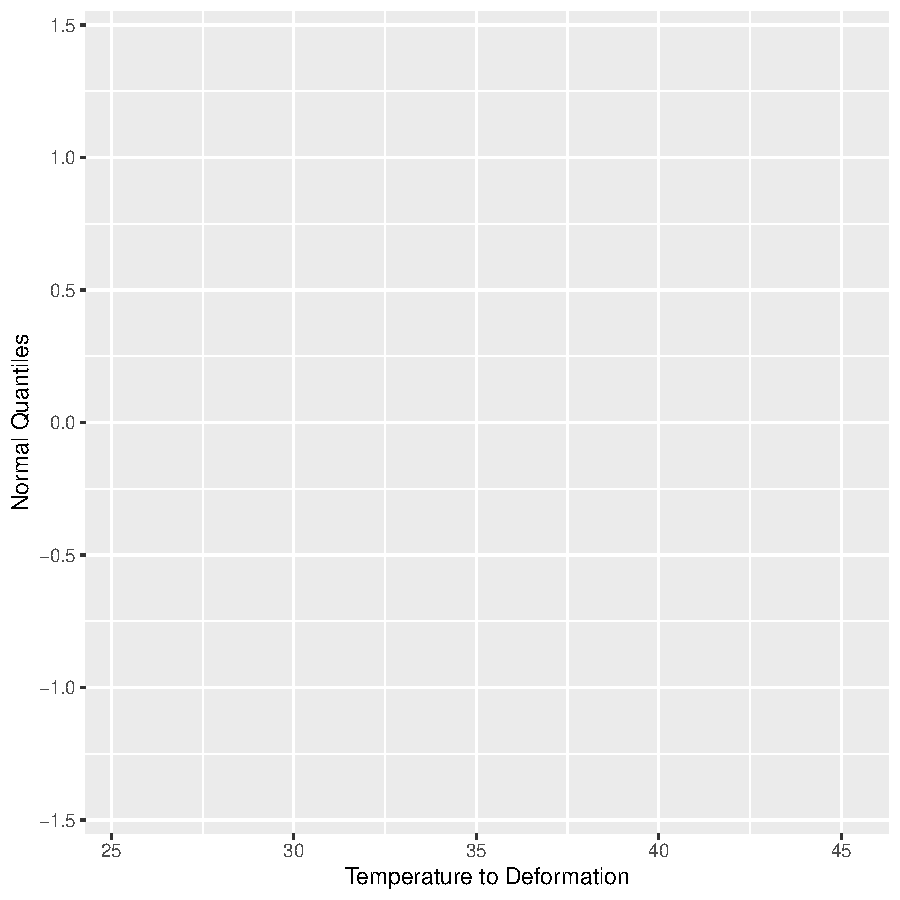
\includegraphics{stat305-exam1-014}

\end{parts}
\pagebreak




\end{questions}

\end{document}
